\section{Method}
\ourmethod consists of three algorithmic components: 1) environment as context that enables zero-shot generation of executable rewards, 2) evolutionary search that iteratively proposes and refines reward candidates, and 3) reward reflection that enables fine-grained reward improvement. See Alg.~\ref{algo:eureka} for pseudocode; all prompts are included in App.~\ref{appendix:full-prompts}. 







\subsection{Environment as Context}
\label{sec:env-as-context}


Reward design requires the environment specification to be provided to the LLM.
We propose directly feeding the raw environment source code (without the reward code, if exists) as context. \arxiv{Given that any reward function is a function over the environment's state and action variables, the only requirement in the source code is that it exposes these environment variables, which is easy to satisfy. In cases where the source code is not available, relevant state information can also be supplied via an API, for example. In practice, to ensure that the environment code fits within the LLM's context window and does not leak simulation internals (so that we can expect the same prompt to generalize to new simulators), we have an automatic script to extract just the environment code snippets that expose and fully specify the environment state and action variables. see App.~\ref{appendix:experimental-details} for details.}





\begin{wrapfigure}{r}{0.6\linewidth}
\begin{minipage}{0.6\textwidth}
\begin{algorithm}[H]
\caption{\ourmethod}
\label{algo:eureka}
\begin{algorithmic}[1]
\small
\STATE \textbf{Require}: Task description $l$, environment code $M$, \\ 
coding LLM $\texttt{LLM}$, fitness function $F$, initial prompt $\texttt{prompt}$
\STATE \textbf{Hyperparameters}: search iteration $N$, iteration batch size $K$
\FOR{\text{N iterations}}
\STATE \textcolor{purple}{\texttt{// Sample $K$ reward code from LLM}}
\STATE $\texttt{R}_1,..., \texttt{R}_k \sim \texttt{LLM}(l, M, \texttt{prompt})$ 
\STATE \textcolor{purple}{\texttt{// Evaluate reward candidates}}
\STATE $s_1 =F(\texttt{R}_1), ..., s_K = F(\texttt{R}_K)$
\STATE \textcolor{purple}{\texttt{// Reward reflection}}
\STATE $\texttt{prompt} := \texttt{prompt} : \texttt{Reflection}(R^n_{best}, s^n_{best})$,\\ 
where $best = \arg \max_{k} s_1,...,s_K$
\STATE \textcolor{purple}{\texttt{// Update Eureka reward}}
\STATE $R_{\text{Eureka}}, s_{\text{Eureka}} = (R^n_{\text{best}}, s^n_{\text{best}})$, \quad if $s^n_{\text{best}} > s_{\text{Eureka}}$
\ENDFOR
\STATE \textbf{Output}: $R_{\text{Eureka}}$
\end{algorithmic}
\end{algorithm}
\end{minipage}
\end{wrapfigure}




\arxiv{Given environment as context}, \ourmethod instructs the coding LLM to directly return executable Python code with only generic reward design and formatting tips, such as exposing individual components in the reward as a dictionary output (for reasons that will be apparent in Sec.~\ref{sec:reward-reflection}); \arxiv{see Prompt 1 and 3 in App.~\ref{appendix:full-prompts}.}
Remarkably, with only these minimal instructions, \ourmethod can already zero-shot generate plausibly-looking rewards in diverse environments in its first attempts. An example \ourmethod output is shown in Fig.~\ref{fig:eureka-reward}. As seen, \ourmethod adeptly composes over existing observation variables (e.g., \texttt{fingertip\_pos}) in the provided environment code and produces a competent reward code -- all without any environment-specific prompt engineering or reward templating. On the first try, however, the generated reward may not always be executable, and even if it is, it can be quite sub-optimal with respect to the task fitness metric $F$. While we can improve the prompt with task-specific formatting and reward design hints, doing so does not scale to new tasks and hinders the overall generality of our system. How can we effectively overcome the sub-optimality of single-sample reward generation?  




\begin{figure*}[t!]
\centering 
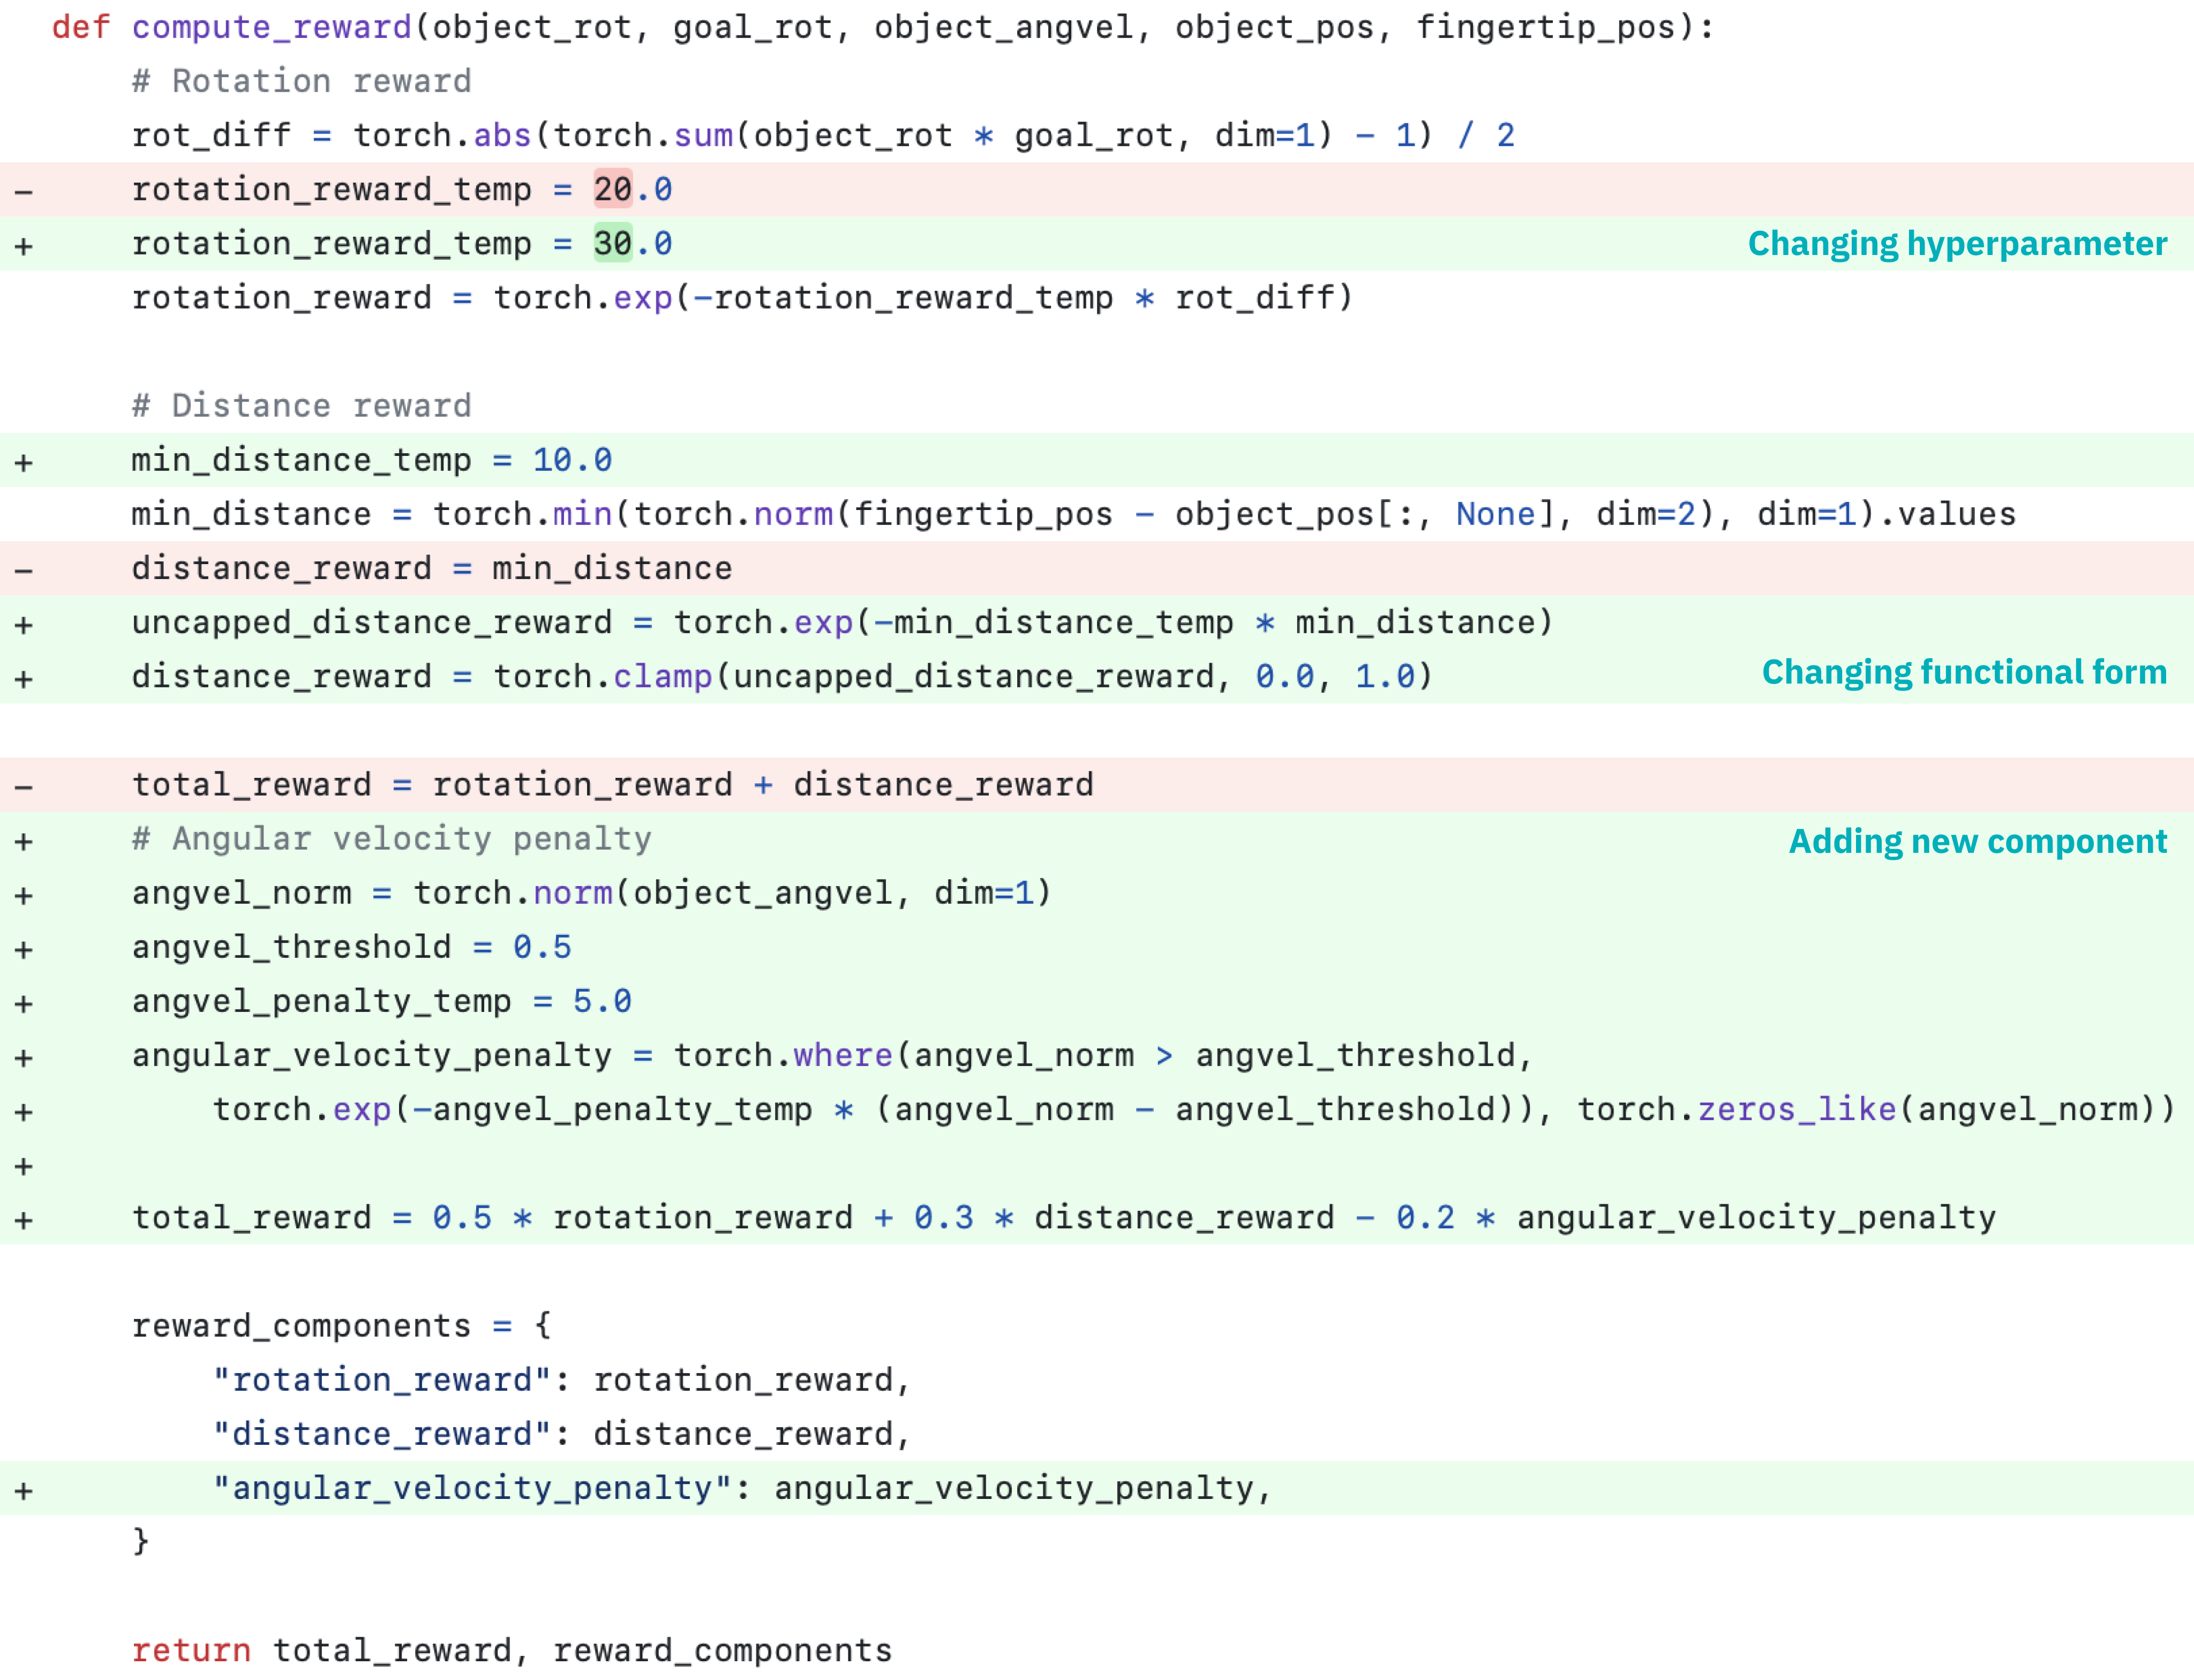
\includegraphics[width=0.8\textwidth]{figures/reward_diff.png}
\caption{\ourmethod can zero-shot generate executable rewards and then flexibly improve them with many distinct types of free-form modification, such as (1) changing the hyperparameter of existing reward components, (2) changing the functional form of existing reward components, and (3) introducing new reward components.}
  \label{fig:eureka-reward}
\end{figure*}

\subsection{Evolutionary Search}
\label{sec:evolutionary-search}

In this section, we will demonstrate how evolutionary search presents a natural solution that addresses the aforementioned execution error and sub-optimality challenges. In each iteration, \ourmethod samples several independent outputs from the LLM (Line 5 in Alg.~\ref{algo:eureka}). Since the generations are i.i.d, the probability that \textit{all} reward functions from an iteration are buggy \textit{exponentially} decreases as the number of samples increases. We find that for all environments we consider, sampling just \arxiv{a modest number of samples (16)} contains at least one executable reward code in the first iteration. 





Given executable reward functions from an earlier iteration, \ourmethod performs in-context \textit{reward mutation}, proposing new improved reward functions from the best one in the previous iteration.
\arxiv{Concretely, a new \ourmethod iteration will take the best-performing reward from the previous iteration, its reward reflection (Sec.~\ref{sec:reward-reflection}), and the mutation prompt (Prompt 2 in App.~\ref{appendix:full-prompts})} as context and generate $K$ more i.i.d reward outputs from the LLM; several illustrative reward modifications are visualized in Fig.~\ref{fig:eureka-reward}. This iterative optimization continues until a specified number of iterations has been reached. Finally, we perform multiple random restarts to find better maxima; this is a standard strategy in global optimization. In all our experiments, \ourmethod conducts 5 independent runs per environment, and for each run, searches for $5$ iterations with $K=16$ samples per iteration.






\subsection{Reward Reflection}
\label{sec:reward-reflection}
In order to ground the in-context reward mutation, we must be able to put into words the quality of the generated rewards. We propose \arxiv{\textit{reward reflection}, an automated feedback that summarizes the policy training dynamics in texts. Specifically, given that \ourmethod reward functions are asked to expose their individual components in the reward program (e.g., \texttt{reward\_components} in Fig.~\ref{fig:eureka-reward}), reward reflection tracks the scalar values of all reward components and the task fitness function at intermediate policy checkpoints throughout training. For instance, consider the illustrative example in Fig.~\ref{fig:eureka-concept}, where the snapshot values of $\texttt{av\_penalty}$ are provided as a list in the reward feedback. See App.~\ref{appendix:reward-reflection-examples} for full examples.}







This reward reflection procedure, though simple to construct, is important due to \arxiv{two reasons: (1) the lack of fine-grained reward improvement signal in the task fitness function, and (2) the algorithm-dependent nature of reward optimization~\citep{booth2023perils}.} First, as we can query the task fitness function $F$ on the resulting policies, a simple strategy is to just provide this numerical score as the reward evaluation. While serving as the holistic ground-truth metric, the task fitness function itself lacks in credit assignment, providing no useful information on \textit{why} a reward function works or not. Second, whether a reward function is effective is influenced by the particular choice of RL algorithm, and the same reward may perform very differently even under the same optimizer given hyperparameter differences~\citep{henderson2018deep, agarwal2021deep}. By providing detailed accounts on how well the RL algorithm optimizes individual reward components, reward reflection enables \ourmethod to produce more intricate and targeted reward editing. 













